%\documentclass[preprint,prl,superscriptaddress]{revtex4-1}
%\documentclass[twocolumn,nofootinbib]{nature}
\documentclass[onecolumn,pra,superscriptaddress,nofootinbib]{revtex4-1}

% packages
\usepackage[dvips]{graphicx} % for figures
\usepackage{amsfonts,amssymb,amscd,amsmath,amsthm}
\usepackage{enumerate}
\usepackage{epsfig}
\usepackage{subfigure}
\usepackage{xcolor}
%\usepackage[expert]{mathdesign}
	

\newcommand{\bra}[1]{\mbox{$\left\langle #1 \right|$}}
\newcommand{\ket}[1]{\mbox{$\left| #1 \right\rangle$}}
\newcommand{\braket}[2]{\mbox{$\left\langle #1 | #2 \right\rangle$}}
\newcommand{\ketbra}[2]{\mbox{$\left\vert #1\right\rangle \left\langle #2\right\vert$ }}
\newcommand{\Tr}{\mathrm{Tr}}
\newcommand{\bfone}{\mathbf{I}}

\newtheorem{theorem}{Theorem}
\newtheorem{lemma}{Lemma}
\newtheorem{corollary}{Corollary}
\newtheorem{claim}{Claim}
\newtheorem{conjecture}{Conjecture}
\newtheorem*{observation}{Observation}
\newtheorem{definition}{Definition}

\begin{document}

\title{Lecture 2: two-qubit system}

%% For REVTeX it is possible to automate superscript and e-mail callouts with the superscriptaddress option; see REVTeX4 documentation.


\author{Xiongfeng Ma}
\email{xma@tsinghua.edu.cn}
\affiliation{Center for Quantum Information, Institute for Interdisciplinary Information Sciences, Tsinghua University, Beijing 100084, China}


\begin{abstract}
In the last chapter, we have learned about one qubit system. Here, we shall learn about a two-qubit system. It turns out two-qubit system has much more fun. It will take three weeks for us to cover these materials. Guess how many qubits we can cover by the end of the course?

Two-qubit state, mixed state, Bloch ``ball", positive-operator valued measure (POVM); Super operator, purification of mixed state and POVM; Using teleportation for operation (Gottesman-Chuang'99), remote state preparation; Bell's inequality, CHSH/CH/Eberhard inequality; experiment development and loopholes, entanglement; Quantum dense coding, teleportation (experiment development);
\end{abstract}

%\ocis{(270.5565) Quantum communications; (270.5568) Quantum cryptography.}


\maketitle %% required

\section{Review: one-qubit System}
\begin{enumerate}
\item{state: ray.}
\item{normalize state: vector.}
\item{representation way: $\ket{u}=\cos{\frac{\theta}{2}}+e^{i\varphi}\sin{\frac{\theta}{2}}$. (Bloch Sphere\footnote{No standard way to visualize two or more qubits system until now.})}
\item{density matrix: $\rho = \sum_i\lambda_i\ket{\phi_i}\bra{\phi_i}$.\footnote{why we can't distinguish $\ket{u}$ and $e^{i\theta}\ket{u}$? because $\ket{u}\bra{u}=e^{i\theta}\ket{u}\bra{u}e^{-i\theta}$. Their density matrices are always the same.}}
\item{$\rho^{+} = \rho, Tr(\rho) = 1.$}
\item{$\forall \ket{\phi}, \bra{\phi}\rho\ket{\phi} \geq 0$.\footnote{By physical meaning of the measurement}}
\item{For pure qubit, Assume $\rho = \ket{\phi}\bra{\phi}$, we have $\rho^2 = \rho.$ Also, we can get the eigenvalues and eigenvectors of $\rho$ (Assume $\ket{\Phi}$ is orthogonal of $\ket{\phi}$):
\begin{equation}
\begin{aligned}
\rho\ket{\phi} = \ket{\phi}\braket{\phi}{\phi} = \ket{\phi}.\\
\rho\ket{\Phi} = \ket{\phi}\braket{\phi}{\Phi} = 0.
\end{aligned}
\end{equation}}

\item{$\bra{\psi}M\ket{\psi} = Tr(\bra{\psi}M\ket{\psi}) = Tr(M\ket{\psi}\bra{\psi}) = Tr(M\rho).$\footnote{$Tr(AB)=\sum_{i}\sum_j a_{ij}b_{ji} = \sum_{i}\sum_j b_{ij}a_{ji} = Tr(BA)$.}}
\end{enumerate}

\section{Notations}
Matrix tensor product $\otimes$,
%consider two matrices,
%\begin{equation} \label{2qubit:2mat}
%\begin{aligned}
%\[
%\begin{pmatrix}
%    a_{1,1} & a_{1,2} \\
%    a_{2,1} & a_{2,2}
%\end{pmatrix}
%
%\begin{pmatrix}
%    b_{1,1} & b_{1,2} \\
%    b_{2,1} & b_{2,2}
%\end{pmatrix}.
%\]
%\end{aligned}
%\end{equation}
the tensor product of two matrices is
\begin{equation} \label{2qubit:tensorproduct}
\begin{aligned}
  \begin{bmatrix}
    a_{1,1} & a_{1,2} \\
    a_{2,1} & a_{2,2} \\
  \end{bmatrix}
\otimes
  \begin{bmatrix}
    b_{1,1} & b_{1,2} \\
    b_{2,1} & b_{2,2} \\
  \end{bmatrix}
=
  \begin{bmatrix}
    a_{1,1}  \begin{bmatrix}
              b_{1,1} & b_{1,2} \\
              b_{2,1} & b_{2,2} \\
            \end{bmatrix} & a_{1,2}  \begin{bmatrix}
                                      b_{1,1} & b_{1,2} \\
                                      b_{2,1} & b_{2,2} \\
                                    \end{bmatrix} \\
     & \\
    a_{2,1}  \begin{bmatrix}
              b_{1,1} & b_{1,2} \\
              b_{2,1} & b_{2,2} \\
            \end{bmatrix} & a_{2,2}  \begin{bmatrix}
                                      b_{1,1} & b_{1,2} \\
                                      b_{2,1} & b_{2,2} \\
                                    \end{bmatrix} \\
  \end{bmatrix}
=
  \begin{bmatrix}
    a_{1,1} b_{1,1} & a_{1,1} b_{1,2} & a_{1,2} b_{1,1} & a_{1,2} b_{1,2} \\
    a_{1,1} b_{2,1} & a_{1,1} b_{2,2} & a_{1,2} b_{2,1} & a_{1,2} b_{2,2} \\
    a_{2,1} b_{1,1} & a_{2,1} b_{1,2} & a_{2,2} b_{1,1} & a_{2,2} b_{1,2} \\
    a_{2,1} b_{2,1} & a_{2,1} b_{2,2} & a_{2,2} b_{2,1} & a_{2,2} b_{2,2} \\
  \end{bmatrix}.
\end{aligned}
\end{equation}


Here, we simplify denote it as
\begin{equation} \label{2qubit:tensorsimp}
\begin{aligned}
\ket{\phi}\otimes\ket{\psi} = \ket{\phi}\ket{\psi}\\
\end{aligned}
\end{equation}


\subsection{Trace}
Trace $Tr(\rho)$: summation of the diagonal terms.

Partial trace $Tr_B(\rho_{AB})$: Assume A is n-dimension state, B is m-dimension state, then $\rho_{AB}$ can be regarded as a $nm \times nm$ matrix. $Tr_B(\rho_{AB})$ is a $n\times n$ matrix, where
\begin{equation} \label{2qubit:partialtr}
\begin{aligned}
(Tr_B(\rho_{AB}))_{ij} = \sum_{k=1}^{m}(\rho_{AB})_{ik, jk} \\
\end{aligned}
\end{equation}
Particularly, $Tr_B(A \otimes B) = Tr(B)A.$



\subsection{Schmidt decomposition}
For any pure state $\ket{\psi}_{AB}$ of a bipartite system, there are orthonormal bases $\{\ket{i}_A\}$ and $\{\ket{i��}_B\}$ such that:
\begin{equation} \label{Schmidt decomposition}
\begin{aligned}
\ket{\psi}_{AB}=\sum_i\sqrt{p_i}\ket{i}_A\otimes\ket{i'}_B.
\end{aligned}
\end{equation}
The subsystems $A$ and $B$ have the same eigenvalues, $p_i$s. The number of $p_i$s is called the Schmidt number of $\ket{\psi}_{AB}$. We denote that the pure state is a entangled state when the the Schmidt number is greater than one. It is easy to see that the Bell states are entangled states.




\section{Two-qubit system}

\subsection{an interesting ``paradox"}
When considering a two qubits state which is written as
\begin{equation} \label{2qubit:4Bell0011}
\begin{aligned}
\ket{\psi}_{AB}=\frac{1}{\sqrt2}(\ket{0}_{A}\ket{0}_{B}+\ket{1}_{A}\ket{1}_{B}).\\
\end{aligned}
\end{equation}
When measure the system $A$ in the $Z$ basis, with probability $1/2$, the measurement result is $\ket{0}$ and the prepared state is $\ket{0}_A\ket{0}_B$. With probability $1/2$, the measurement result is $\ket{1}$ and the prepared state is $\ket{1}_A\ket{1}_B$. Naively, one might express system $A$ in the state of
\begin{equation} \label{2qubit:plus}
\begin{aligned}
\ket{\psi}_A = \frac{1}{\sqrt{2}}(\ket{0} + \ket{1}) = \ket{+}.
\end{aligned}
\end{equation}


Consider another two-qubit state,
\begin{equation} \label{2qubit:4Bellppmm}
\begin{aligned}
\ket{\psi}_{AB}=\frac{1}{\sqrt2}(\ket{+}_{A}\ket{+}_{B}+\ket{-}_{A}\ket{-}_{B}).\\
\end{aligned}
\end{equation}
Following the same naive argument, we should have
\begin{equation} \label{2qubit:0}
\begin{aligned}
\ket{\psi}_A = \frac{1}{\sqrt{2}}(\ket{+} + \ket{-}) = \ket{0}.
\end{aligned}
\end{equation}

But, on the other hand,
\begin{equation} \label{2qubit:Belleq}
\begin{aligned}
\ket{\psi}_{AB}&=\frac{1}{\sqrt2}(\ket{0}_{A}\ket{0}_{B}+\ket{1}_{A}\ket{1}_{B}) \\
 &= \frac{1}{2\sqrt2}(\ket{+}+\ket{-})(\ket{+}+\ket{-})+\frac{1}{2\sqrt2}(\ket{+}-\ket{-})(\ket{+}-\ket{-})\\
 &= \frac{1}{\sqrt2}(\ket{+}_A\ket{+}_B+\ket{-}_A\ket{-}_B).
\end{aligned}
\end{equation}
So now we have: $\ket{0} = \ket{+}$. What is wrong?


\textbf{Explanation:} The key of the above paradox is that $\ket{\psi}_A$ is not a pure state any more, we only can write it as a density matrix. The density operator of subsystem A is given by
\begin{equation} \label{4BellZ}
\begin{aligned}
\rho_A=tr_B(\ket{\psi}_{AB}\bra{\psi}_{AB})=\frac{1}{\sqrt{2}}(\ket{0}\bra{0}+\ket{1}\bra{1}).\\
\end{aligned}
\end{equation}


\subsection{EPR paradox}
Alice and Bob share a two qubits system:
$$
\ket{\psi}_{AB} = \frac{1}{\sqrt2}(\ket{0}_{A}\ket{0}_{B}+\ket{1}_{A}\ket{1}_{B}).
$$
Alice gets qubit A, Bob gets qubit B. Then Alice goes to a planet which far from Bob. Then if Alice wants to tell 0 to B, she measures A in $\ket{+/-}$ basis; if she wants to tell 1 to B, she measures A with $\ket{0/1}$ basis.

We assume that after measurement for A, Alice gets $\ket{0}$. Then
for Bob, he measures B after a while with basis $\ket{0/1}$, if he gets $\ket{0}$ with probability 1, he can say Alice wants to tell him 0.

So by this process, we transform information which is faster than light. What's the problem?

\textbf{Explanation:} For Bob, if he gets $\ket{0}$, he doesn't know which basis Alice uses. Because if Alice chooses $\ket{0/1}$ basis, Bob has $0.5$ probability to get $\ket{0}$; if Alice chooses $\ket{+/-}$ basis, Bob also has $0.5$ probability to get $\ket{0}$.

This experiments tells us, quantum has the \textbf{non-locality} and also \textbf{no-signalling} properties.
$$
\textit{Something are changed, but we do not know. We simply use the same state to describe the system.}
$$



\subsection{The properties for general density matrix}
In general, the state is represented by a density operator.
In the case where the state of the subsystem is a ray, and we say that the state is
pure. Otherwise the state is mixed. If $\rho_A=\rho_A^2$, then $\ket{\psi_A}$ is a pure state. Otherwise, the density matrix of A is
$\rho_A=\sum_a p_a\ket{a}\bra{a}$, where $\sum_ap_a=1$, $0<p_a<1$. The trace distance $tr \rho_A^2=\sum_a p_a^2<\sum_ap_a=1$.

Properties of a general density matrix
\begin{enumerate}
\item
self-adjoint: $\rho_A=\rho_A^\dag$
\item
positivity: $\forall\ket{\psi}$, $\bra{\psi}\rho_A\ket{\psi}\ge0$
\item
completeness: $Tr(\rho_A)=1$
\end{enumerate}



\subsection{Schmidt decomposition}
For any pure state $\ket{\psi}_{AB}$ of a bipartite system, there are orthonormal bases $\{\ket{i}_A\}$ and $\{\ket{i��}_B\}$ such that:
\begin{equation} \label{Schmidt decomposition}
\begin{aligned}
\ket{\psi}_{AB}=\sum_i\sqrt{p_i}\ket{i}_A\otimes\ket{i'}_B.
\end{aligned}
\end{equation}
The subsystems $A$ and $B$ have the same eigenvalues, $p_i$s. The number of $p_i$s is called the Schmidt number of $\ket{\psi}_{AB}$. We denote that the pure state is a entangled state when the the Schmidt number is greater than one. It is easy to see that the Bell states are entangled states.


%% week3
For pure $\ket{\psi}_{AB} = \sum\sqrt{p_i}\ket{i}\bra{i'}$, you can always find $\rho_A = \rho_B$ in all basis ($\rho_A = \Tr_B(\psi_{AB})$)


\subsection{Bell basis}
The dimension of the 2-qubit Hilbert space is 4. Thus, there are 4 basis states. Bell state basis is widely used, especially for the case involving entanglement. The 4 Bell states in the $Z$ basis are,
\begin{equation} \label{4BellZ}
\begin{aligned}
\Phi^+ &= \ket{00}+\ket{11} \\
\Phi^- &= \ket{00}-\ket{11} \\
\Psi^+ &= \ket{01}+\ket{10} \\
\Psi^- &= \ket{01}-\ket{10} \\
\end{aligned}
\end{equation}
in the $X$ basis are
\begin{equation} \label{4BellZ}
\begin{aligned}
\Phi^+ &= \ket{++}+\ket{--} \\
\Phi^- &= \ket{-+}+\ket{+-} \\
\Psi^+ &= \ket{++}-\ket{--} \\
\Psi^- &= \ket{-+}-\ket{+-} \\
\end{aligned}
\end{equation}
in the $Y$ basis are
\begin{equation} \label{4BellZ}
\begin{aligned}
\Phi^+ &= \ket{+i-i}+\ket{-i+i} \\
\Phi^- &= \ket{+i+i}+\ket{-i-i} \\
\Psi^+ &= -i(\ket{+i+i}-\ket{-i-i}) \\
\Psi^- &= i(\ket{+i-i}-\ket{-i+i}) \\
\end{aligned}
\end{equation}

Many interesting simple quantum information phenomenons come with Bell states, such as Bell's inequality, Teleportation, super dense coding, quantum key distribution, and Deutsch's algorithm.


\subsection{Bloch sphere and qubit tomography}
A useful representation of the state of a single qubit is the Bloch sphere representation. Since the overall phase is irrelevant, a pure state of a qubit can be written as
\begin{equation} \label{eq:BlochSphere}
\begin{aligned}
\ket{u} = \cos\frac{\theta}{2}\ket{0}+e^{i\varphi}\sin\frac{\theta}{2}\ket{1}.
\end{aligned}
\end{equation}
Therefore, it is convenient to represent it as a vector living the surface of a unit sphere with the spherical coordinate $(r=1,\theta,\varphi)$.

\begin{figure}[tbh]
\centering \resizebox{4cm}{!}{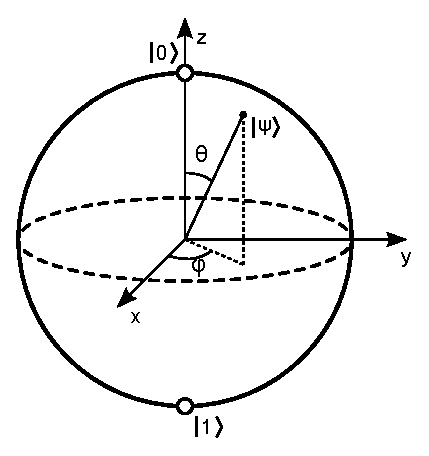
\includegraphics{epsBlochSphere.eps}}
\caption{Bloch sphere.} \label{fig:BlochSphere}
\end{figure}

In general, a qubit might be in a mixed state, and then it will be within the Bloch sphere instead on the surface. In general, the density matrix of a qubit can be written as
\begin{equation} \label{eq:rhoBloch}
\begin{aligned}
\rho &= \frac12(\sigma_0+\vec{P}\cdot \vec{\sigma}) \\
&= \frac12
    \begin{pmatrix}
      1+P_z&P_x-iP_y\\
      P_x+iP_y&1-P_z
    \end{pmatrix}
\end{aligned}
\end{equation}
where $\vec{P}=(P_x,P_y,P_z)$ is a vector and $|\vec{P}|\le1$. When $|\vec{P}|=1$, Eq.~\eqref{eq:rhoBloch} represents a pure qubit.

Quantum state tomography is the process of reconstructing the quantum state for a quantum system by proper measurements. The quantum state can be pure (vector) or in general mixed (density matrix). A set of measurements is called tomographically complete if it can uniquely identify the state. That is, the measurement outcomes are able to provide all the information about the state. In the classical physics, it corresponds to system calibration.

Let us take qubit tomography for example. As given in Eq.~\eqref{eq:rhoBloch}, the $Z$ basis measure provides the information on $P_z$. By changing the $Z$ and $X$ basis, by the Hadamard transformation, we can conclude that the $X$ basis measure provides the information on $P_x$. Similarly, the $Y$ basis measure provides the information on $P_y$. Thus, $X$, $Y$, and $Z$ measurements is tomographically complete for a qubit. Another way to put this is,
\begin{equation} \label{eq:rho2tomo}
\begin{aligned}
\rho &= \frac12[tr(\rho)\sigma_0+tr(\sigma_x\rho)\sigma_x+tr(\sigma_y\rho)\sigma_y+tr(\sigma_z\rho)\sigma_z]. \\
\end{aligned}
\end{equation}
Now, let us move a bit further, tomography for $n$ qubits,
\begin{equation} \label{eq:rhontomo}
\begin{aligned}
\rho &= 2^{-n}\sum_{v_1,v_2,\dots,v_n\in\{0,x,y,z\}}tr(\sigma_{v1}\otimes\sigma_{v2}\otimes\cdots\otimes\sigma_{vn}\rho) \sigma_{v1}\otimes\sigma_{v2}\otimes\cdots\otimes\sigma_{vn},
\end{aligned}
\end{equation}
where the sum is over all possible the identity and Pauli matrices.

In another related concept, quantum process tomography, known quantum states are used to probe a quantum process to find out how the process can be described. Similarly, quantum measurement tomography works to find out what measurement is being performed.

The general principle behind quantum state tomography is that by repeatedly performing many different measurements on quantum systems described by identical density matrices, frequency counts can be used to infer probabilities, and these probabilities are combined with Born's rule to determine a density matrix which fits the best with the observations.



%%%%%%%%%%
%% From week2-2
\begin{itemize}
\item $\rho_A = \Tr_B(\rho_{AB})$, e.g. $\vert\psi\rangle_{AB} = a\vert 0\rangle_A \vert 0\rangle_B + b \vert 1\rangle_A \vert 1\rangle_B$. Then $\rho_A = \Tr_B(\vert\psi\rangle_{AB}\langle\psi\vert_{AB}) = aa^* \vert 0\rangle \langle 0\vert + bb^*\vert 1\rangle \langle 1\vert$ 
\item Property: (1)$\rho_A^\dagger = \rho_A$; (2)$\rho_A\geq 0$(when diagonalized) (3)$\Tr(\rho_A) =1 $ (pure state)

Comment: If $\rho_A$ is pure state, then $\rho_A^2 = \rho_A$, the purity $\Tr(\rho_A^2)\leq 1 \Rightarrow \Tr(\rho_A^2) =1 $.
\item Pauli matrices: $\sigma_x,\sigma_y,\sigma_z,\mathbf{I}$. $\rho = \frac{1}{2}(\mathbf{I}+\vec{P}\cdot \vec{\sigma})$. $\vec{P}\cdot\vec{\sigma} = P_x\sigma_x + P_y\sigma_y+P_z\sigma_z$.

Special case: $\rho = \frac12 (\bfone+\sigma_z) = \vert 0\rangle \langle 0\vert , \frac12 (1-\sigma_z) = \vert 1\rangle \langle 1\vert$.
$\frac12 (\bfone \pm\sigma_x) = \vert \pm\rangle, \frac12 (1\pm\sigma_y) = \vert \pm i\rangle$.
\item We can get $\vert \vec{P}\vert\leq 1$ from $\rho\leq \bfone$. $\vert \vec{P}\vert = 1 $ means pure state, $\vert \vec{P}\vert<1$ means mixed state.
\end{itemize}

\subparagraph{}
$\vert\psi\rangle_{AB} =  \vert 0\rangle_A \vert 0\rangle_B+\vert 1\rangle_A\vert 1\rangle_B = \vert+\rangle_A\vert +\rangle_B+\vert - \rangle_A\vert -\rangle_B$ has two representations. There are two cases to measure $\rho_A = \frac12 \bfone$.
\subparagraph{Case 1:} How to get $\rho_A = \frac12 ( \vert 0\rangle \langle 0\vert+\vert 1\rangle\langle 1\vert)$ ?
\begin{enumerate}

\item Prepare $\vert0\rangle\vert 0\rangle+\vert 1\rangle\vert 1\rangle$
\item Measure $B$ in $z=0$ and $z=1$
\item Given $z$-measure result. $A=\vert 0\rangle$ or $\vert 1\rangle$.
\end{enumerate}
\subparagraph{Case 2: } How to get $\rho_A = \frac12 (\vert+\rangle\langle +\vert+\vert - \rangle\langle -\vert)$?
\begin{enumerate}
\item Prepare $\vert+\rangle\vert +\rangle+\vert - \rangle\vert -\rangle$
\item measure $B$ in $x = \vert +\rangle$ and $x= \vert -\rangle$.
\item Given $x$-measure results, $A = \vert +\rangle$ or $\vert -\rangle$
\end{enumerate}

\subparagraph{}
Using classical coins, Alice prepare the qubits for Bob.

1': Flip a coin, Head or Tail. prepare qubit $\vert 0\rangle$ or $\vert 1\rangle$, then $\rho_{1'} = \frac12 \vert 0\rangle\langle 0\vert +\frac12 \vert 1\rangle\langle 1\vert$

1'',Flip a coin, prepare qubit $\vert +\rangle$ or $\vert -\rangle$, $\rho_{1''} = \frac12 \vert +\rangle\langle +\vert +\frac12 \vert -\rangle\langle -\vert$.

Then $\rho_{1'} = \rho_{1''}$. From Bob's point of view, they are the same, although  Alice knows which of the two pure states it is. When Alice tells Bob the information of the state, the states collapses. (Information is physical; physics is informational.)

Comment:  Given a pure state, we know every information in the system and can not change it by getting more information, since the entropy is already zero (not the case for general density matrix).

\subparagraph{Coherence (classical mixture or superposition).}
 $\vert\psi\rangle = \frac{1}{\sqrt2}(\vert 0\rangle+\vert 1\rangle), \vert \psi\rangle \langle \psi\vert = \frac12 \left[\begin{array}{cc}1 & 1\\1& 1\end{array}\right]$. If we measure in $x$ we always get the same.
But it is different for $\frac12 \vert 0\rangle\langle 0\vert +\frac12 \vert 1\rangle\langle 1\vert$ (which can be distinguished by measuring in $z$).

We prefer the pure state $\frac{1}{\sqrt2}(\vert 0\rangle+\vert 1\rangle)$ to generated randomness, because additional information can not change the state, while the other one can be attacked by measuring the entangled qubit.




\section{Positive Operator-Valued Measure}
For the bipartite state $\ket{\psi}_{AB}$,
\begin{equation} \label{2qubit:2qubiteg}
\begin{aligned}
\ket{\psi}_{AB}=a \ket{0}_{A}\ket{0}_{B}+b\ket{1}_{A}\ket{1}_{B}, \\
\end{aligned}
\end{equation}
if we only measure system $A$, the observable can be expressed as
\begin{equation} \label{2qubit:jointmeasure}
\begin{aligned}
M_A\otimes I_B
\end{aligned}
\end{equation}
where $M_A$ is a self-adjoint operator acting on system $A$. Then the expectation value of the measurement outcome is,
\begin{equation} \label{2qubit:jointmeasureExp}
\begin{aligned}
\bra{\psi}M_A\otimes I_B\ket{\psi} &= (a^* \bra{0}_{A}\bra{0}_{B}+b^*\bra{1}_{A}\bra{1}_{B}) (M_A\otimes I_B) (a \ket{0}_{A}\ket{0}_{B}+b\ket{1}_{A}\ket{1}_{B}) \\
&= |a|^2 \bra{0}M_{A}\ket{0}+|b|^2\bra{1}M_{A}\ket{1}. \\
\end{aligned}
\end{equation}
Since we know that the density matrix of $\rho_A=|a|^2\ket{0}\bra{0}+|b|^2\ket{1}\bra{1}$, Eq.~\eqref{2qubit:jointmeasureExp} can be written as,
\begin{equation} \label{2qubit:jointmeasureExprho}
\begin{aligned}
\langle M_A \rangle = tr(M_A\rho_A)
\end{aligned}
\end{equation}

We can understands the difference between the Positive Operator-Valued Measure (POVM) and PVM with the same sense that a density matrix is to a pure state.  The POVM can be used to describe the effect of PVM acts on a large system.
The operators $\{E_a\}$ form a complete set of Hermitian nonnegative operators and satisfy that:
\begin{enumerate}
\item Hermiticity: $E_a=E_a^\dag$.
\item Positivity :$\bra{\psi}E_a\ket{\psi}\ge0$.
\item Completeness: $\sum_aE_a=I$.
\end{enumerate}

%% From week2-2

\subsection{State tomography}
How to measure $\rho = \frac12 = (I+\vec{P}\cdot\vec{\sigma})$?
\subparagraph{Measure states by PVM:}
$\vert\psi\rangle_{AB} = a\vert 00\rangle+b\vert11\rangle$. $M_A\otimes I$. 
The expectation 
\begin{eqnarray*}
\langle M_A\otimes I\rangle &= &\Tr(M_A\otimes I \vert \psi\rangle \langle\psi\vert) \\
&=& _{AB}\langle\psi\vert M_A\otimes I_B\vert \psi\rangle_{AB} \\
&=&\vert a\vert^2 \langle 0\vert M_A\vert 0\rangle +\vert b\vert^2 \langle 1\vert M_A\vert 1\rangle = \Tr(\rho_A M_A)
\end{eqnarray*}
\subparagraph{Measure density matrix by POVM:}
Expectation $\langle M\rangle = \Tr(M\rho)$.

$\{E_a\}$, (1) $E_a = E_a^\dagger$; (2) $\forall \vert\psi\rangle, \langle\psi\vert E_a\vert\psi\rangle\geq 0$;(3) $\sum_a E_a = 1$.

The probability to get $a$ is $\Tr(E_a\rho)$.
e.g. PVM, qubit, $z$-basis, $a = 0,1$. $E_0 = \vert 0\rangle\langle 0\vert , E_1 = \vert 1\rangle \langle1\vert$.

PVM is the special case of POVM.
\subsection{Measurement}
Many copies (the system reproduces the same state).

Measure in $x$-basis: $+, -$, $\Pr(\pm) = \Tr(\rho E_\pm) = \langle\pm\vert \rho\vert \pm\rangle = \frac12(1 \pm P_x)$ (since $\vert \pm \rangle$ is the eigen state of $\sigma_x$ and $\sigma_x$ is orthogonal to both $\sigma_y$ and $\sigma_z$).

$\Pr(\pm i) =  \frac12(1\pm P_y), \Pr(0/1) = \frac12(1\pm P_z)$.

How to measure arbitrary many qubit? 

$\rho = \sum_x p(x)\ketbra{x} \otimes f(x)$, e.g. $\frac12 \left[ \ketbra{0} \otimes \rho_0 + \ketbra{1}\otimes \rho_1\right]$.

Measure $x,y,z$ for $\rho = \frac12 (I+\vec{P}\cdot\vec{\sigma})$. $P_i = \Tr(\rho\sigma_i)(i = x,y,z)$.
\begin{gather*}
\rho = \frac12 \left( \Tr(\rho I)I + \sum_{i=x,y,z}\Tr(\sigma_i \rho)\sigma_i\right)
\end{gather*}

\subparagraph{two-qubit system.}
Use $\sigma_i\otimes\sigma$ to measure $\rho_{AB}$. 

For $\frac{1}{\sqrt2}(\ket{00}_{AB}\pm \ket{11}_{AB}), \frac{1}{\sqrt2}(\ket{01}\pm\ket{10})$ (can not be written as tensor product),

$\rho_A = \frac{1}{2}[1 0; 0 1] = \rho_B, \rho_{AB} = \rho_A\otimes\rho_B = \left(\begin{array}{cccc}
&&&\\
&&&\\
&&&\\
&&&
\end{array}\right)_{4\times 4} = \sum_{i,j\in\{I,x,y,z\}}P_{ij}\sigma_i\otimes\sigma_j$.


Beccause $\Tr{\rho_{AB}} = \sum_{i,j}P_{ij}\Tr{\sigma_i\otimes\sigma_j} = P_{II}\Tr(\sigma_I)\Tr(\sigma_I) = 4P_{II}=1$, $P_{II} = \frac14$.

$P_{ij} = \Tr(\sigma_{i'j'}P_{i'j'}(\sigma_{i'}\otimes\sigma_{j'})(\sigma_i\otimes\sigma_j)) = \Tr(\rho\sigma_i\otimes\sigma_j)$.

\subparagraph{n-qubit system.}
$\bigotimes_{v_i=\in\{I,x,y,z\}} \sigma_{v_i}, \rho = \sigma_{v_i}\Tr(\rho\bigotimes_{v_i}\sigma_{v_i})\bigotimes(\sigma_{v_i}).$
$3^n$ measurement should be performed, but the DOF is less, so this tomography is not optimal. 

\subparagraph{Individual measurement:} $4^n$ terms (nothing for $I$).
\subparagraph{Joint measurement (BSM: Bell-state measurement):} $\phi^{\pm} = \ket{00}\pm\ket{11}, \psi^{\pm} = \ket{01}\pm\ket{10}$

Hamard $H = \frac{1}{\sqrt2}[1, 1; 1, -1]$ operation, C-NOT operation (control-NOT, flip target qubit when input control qubit $\ket{1}$, e.g. $\ket{1}\ket{0}\mapsto\ket{1}\ket{1})$) is $4\times 4$ unitary matrix:
\begin{gather*}
\left(\begin{array}{cccc}
1&0&0&0\\
0&1&0&0\\
0&0&0&1\\
0&0&1&0
\end{array}\right).
\end{gather*}
$\ket{00}+\ket{11}\underrightarrow{C-NOT}\ket{+}\ket{0} \underrightarrow{H\times I} \ket{0}\ket{0}$, 

$\ket{00}-\ket{11}\underrightarrow{C-NOT, H\otimes I} \ket{1}\ket{0}$, 

$\ket{01}+\ket{10}\mapsto \ket{0}\ket{1}, \ket{01}-\ket{10}\mapsto \ket{1}\ket{1}$, 

$\ket{00}\mapsto\ket{+}\ket{0}$. 

Then measure in $z$-basis.






\section{quantum channel}
The quantum channel is also called ``super operator". The super means that the map takes operators to operators, rather than vectors to vectors. Unitary evolution on $\mathcal{H}_A\otimes\mathcal{H}_B $ will not in general appear to be unitary if we restrict our attention to $\mathcal{H}_A$ alone. Rather, evolution in HA will be described by a quantum channel, (which can be inverted by another channel only if unitary). A general channel $\mathcal{E}$ has an operator-sum representation:
\begin{equation} \label{eq:channel}
\begin{aligned}
\mathcal{E}(\rho)=\sum_aM_a\rho M_a^\dag,\\
\sum_aM_a^\dag M_a=I.\\
\end{aligned}
\end{equation}


\section{Ensembles and purification}
A mixed state of a system A can be prepared as an ensemble of pure states in
many different ways, all of which are experimentally indistinguishable if
we observe system A alone.
\begin{equation} \label{eq:Ensembles}
\begin{aligned}
\rho_A &=\sum_ip_i\ket{\psi_i}\bra{\psi_i}, \\
\end{aligned}
\end{equation}
with $\sum p_i=1$.

For any such $\rho_A$,  we can construct a ``purification" of $\rho_A$, $\ket{\Psi_1}_{AB}$,
\begin{equation} \label{eq:purification}
\begin{aligned}
\ket{\Psi_1}_{AB}=\sum_i \sqrt{p_i}\ket{\psi_i}_A\ket{\alpha_i}_B,
\end{aligned}
\end{equation}
where $\{\ket{\alpha_i}_B\}$ are mutually orthogonal and normalized.

The relation between two purifications, $\ket{\Psi_1}_{AB}$ and $\ket{\Psi_2}_{AB}$, is given by,
\begin{equation} \label{eq:purifications}
\begin{aligned}
\ket{\Psi_1}_{AB}=(I_A\otimes U_B)\ket{\Psi_2}_{AB},
\end{aligned}
\end{equation}
the two states differ by an unitary change of basis acting in $\mathcal{H}_B$ alone.


Given $\rho_A = \frac{1}{2}(\ketbra{0}+\ketbra{1})$, find $\Psi_{AB}$ s.t. $\Tr_{AB} = \rho_A$. Answer: $\ket{00}+\ket{11}$, not unique, but all purification can be linked by linear operation. e.g.
$ \left(\begin{array}{cc}
\frac49 &\frac{1}{100}\\
\frac{1}{100}&\frac59\\
\end{array}\right)$

For diagonal terms, $\sqrt{\frac49}\ket{0}\ket{0}+\sqrt{\frac59}\ket{1}$. For general matrix, extends $\rho_A$ to pure $\rho_{AB}$.
Choose a basis such that $\ket{\psi_{AB}} = \sum \sqrt{x_i}\ket{i}_A\ket{i}_B$ is diagonalized.

Denote eigenvalues of $\rho$ as $\lambda_0,\lambda_1$, eigen states $\ket{\psi_0}, \ket{\psi_1}$. $\rho' = \mathrm{diag}(\lambda_0,\lambda_1)$. $\rho = \lambda_0\ketbra{\psi_0}{\psi_0}+\lambda_1\ketbra{\psi_0}{\psi_0}$, then $\phi_{AB} = \lambda_0\ket{\psi_0}_A\ket{0}_B+\\lambda_1\ket{\psi_1}_A\ket{1}_B$. Comment: Given any mixed states, you can always find a larger Hilbert space such that the density matrix is purified (not unique, but there are relations between such purification).





\section{Bell's inequalities}
Bell's theorem \cite{bell1964einstein}: no physical theory of local hidden variables can ever reproduce all of the predictions of quantum mechanics.
%% week3-2
Refer to Jhon Preskill notes, Hoi-Kwong Lo notes. Local hidden variables can not express any quantum outcomes. Randomness is in the nature of quantum mechanics.



\subsection{Clauser-Horne-Shimony-Holt inequality}
One of the most well known Bell's inequality is the Clauser-Horne-Shimony-Holt (CHSH) inequality \cite{Clauser1969CHSH}. There are many ways to express it. We study it from a quantum game point of view.

As shown in Fig.~\ref{Fig:BellTest}, two space-like separated parties, Alice and Bob, randomly choose input bit settings $x$ and $y$ and generate outputs bits $a$ and $b$ based on their inputs and pre-shared quantum ($\rho$) and classical ($\lambda$) resources, respectively. The probability distribution $p(a,b|x,y)$,  obtaining outputs $a$ and $b$ conditioned on inputs $x$ and $y$, are determined by specific strategies of Alice and Bob. By assuming that the input settings $x$ and $y$ are chosen fully randomly and equally likely, the CHSH inequality is defined by a linear combination of the probability distribution $p(a,b|x,y)$ according to
\begin{equation}\label{eq:Bell}
  S = \sum_{a,b,x,y} (-1)^{a\oplus b + x\cdot y}p(a,b|x,y) \leq S_C = 2,
\end{equation}
where the plus operation $\oplus$ is modulo 2, $\cdot$ is numerical multiplication, and $S_C$ is the (classical) bound of Bell value $S$ for all LHVMs.

\begin{figure}[hbt]
\centering \resizebox{4cm}{!}{\includegraphics{epsBell1.eps}}
\caption{Bipartite Bell inequality. The inputs of Alice and Bob, $x$ and $y$,  are decided by perfect random number generators (RNGs), which produce uniformly distributed random numbers.} \label{Fig:BellTest}
\end{figure}

Similarly, there is an achievable bound $S_Q = 2\sqrt{2}$ for the quantum theory \cite{cirel1980quantum}. In this case, a violation of the classical bound $S_C$ indicates the need for alternative theories other than LHVMs, such as quantum theory. For general no signalling (NS) theories \cite{prbox}, denote the corresponded upper bound as $S_{NS} = 4$. It is straightforward to see that $S_{NS} \geq S_Q\geq S_C$.

Different strategies impose different constraints on the probability distribution.
\begin{itemize}
  \item Classical: $p(a,b|x,y) = \sum_\lambda q(\lambda)p(a|x,\lambda)p(b|y,\lambda)$
  \item Quantum: $p(a,b|x,y) = \mathrm{Tr}[\rho_{AB}M_a^x\otimes M_b^y]$
  \item No-signaling: $\sum_a p(a,b|x,y) = \sum_a p(a,b|x',y), \sum_b p(a,b|x,y) = \sum_b p(a,b|x, y')$
\end{itemize}
\subsection{Experiment loopholes}
Since the first experiment in the early 1980s \cite{Aspect1982PhysRevLett.49.91}, lots of lab demonstrations of the CHSH inequality have been presented. In practice, the conclusion of the violation of a Bell test is conditioned on several assumptions. %\subsection{Experiment problems}
Experimental demonstrations suffer from three major loopholes.

\emph{Locality loophole:}
The measurement events of Alice and Bob should be space-like separated. If this condition is not satisfied, Bell's inequality can be violated even with LHVMs by signaling. This loophole can be closed by separating Alice and Bob sufficient apart such that the measurement events are space-like separated. In experiment, this loophole is closed in optical systems \cite{Weihs98} and shown to be promising to be closed in atomic systems \cite{hofmann2012heralded}.

\emph{Efficiency loophole:}
The detection efficiency must be higher than a threshold to ensure the violation without assuming fair sampling. In the famous CH or Eberhard \cite{Eberhard93} test, it is shown that the efficiency should be at least 2/3 for each party, which is also proved to be a tight bound \cite{Massar03, Wilms08} for all bipartite Bell test with two inputs. The efficiency loophole can be closed in different realizations \cite{rowe2001experimental,Christensen13,giustina2013bell}.

\emph{Randomness loophole:}
The inputs $x$ and $y$ should be random and thus cannot be predetermined. Also, we require $x$ and $y$ to be uncorrelated to each other and also from different runs \cite{Koh12, Pope13}. In experiment, this loophole cannot be closed perfectly, as we can never unconditionally certify the randomness without a faithful Bell test, which in turn requires faithful randomness. Thus, we have to assume the existence of a true random seed. In practice, we can make use of independent random number generators, such as causally disconnected cosmic photons \cite{Gallicchio14}. On the other hand, if we can characterize the randomness well, we can also check whether the input randomness satisfy the requirement \cite{Hall10,Koh12,Pope13,Yuan15,Yuan15b} that guarantee the conclusion even with imperfect randomness input.


\subsection{CH and Eberhard's inequality}
In the bipartite scenario, a general Bell test can be defined as
\begin{equation}\label{Eq:Bellinequality}
  J = \sum_{a,b,x,y} c_{a,b,x,y}p(a,b|x,y) - J_C \geq 0.
\end{equation}
Here, $J_C$ is the classical upper bound and we assume that the probability of choosing $x$ and $y$ is uniform. In practice, a Bell inequality contains both valid outputs such as $o$ $e$ and undetected events $u$, as shown in Fig.~\ref{Fig:CH}. If we take the undetected events into account, the CHSH inequality is defined by the CH or Eberhard's inequality.

\begin{figure}[htb]
  \centering
  % Requires \usepackage{graphicx}
  \resizebox{5cm}{!}{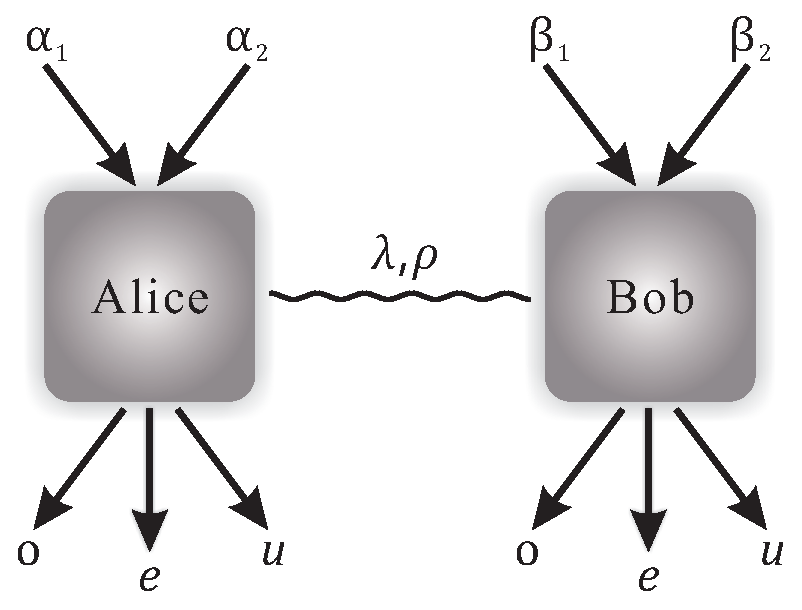
\includegraphics[scale=1]{epsCH.eps}}\\
  \caption{The CH inequality with two input settings and three possible outputs.}\label{Fig:CH}
\end{figure}

\paragraph{CH inequality:}
The CH inequality is a bipartite Bell inequality with measurement settings $x\in\{\alpha_1, \alpha_2\}$ and $y\in\{\beta_1, \beta_2\}$, and outputs $a,b\in\{o,e,u\}$, corresponding to ordinary, extraordinary, and undetected events, respectively. The CH inequality is defined by a linear combination of the probability distribution $p(a,b|x,y)$ by
\begin{equation}\label{eq:CHdef}
\begin{aligned}
  \bar{J} &= -p_{oo}(\alpha_1, \beta_1)  -p_{oo}(\alpha_1, \beta_2) -p_{oo}(\alpha_2, \beta_1)\\
  & +p_{oo}(\alpha_2, \beta_2)+ p_o^A(\alpha_1)  +p_o^B(\beta_1)  \geq 0.
   \end{aligned}
\end{equation}
Here, we take a more convenient notation of $p(a,b|x,y)$ as $p_{ab}(x,y)$, and $p_o^A(\alpha_1)$ ($p_o^B(\beta_1)$) refers to the probability of obtaining $o$ when Alice's (Bob's) input is $\alpha_1$ ($\beta_1$). It is easy to prove that the CH inequality is satisfied with all LVHMs.

In practice, we have to run many times to sample the probability distribution in Eq.~\eqref{eq:CHdef}. Suppose that the input setting is uniformly random and the number of each input setting is $N$, then the CH inequality can also be written as
\begin{equation}\label{eq:CH2}
\begin{aligned}
  N\bar{J} &\approx -n_{oo}(\alpha_1, \beta_1)  -n_{oo}(\alpha_1, \beta_2) -n_{oo}(\alpha_2, \beta_1) \\& +n_{oo}(\alpha_2, \beta_2)+ n_o^A(\alpha_1)/2  +n_o^B(\beta_1)/2  \geq 0.
   \end{aligned}
\end{equation}
Here, $n_{oo}(x, y)$ denotes coincidence detection of $oo$ with inputs $x$ and $y$, and  $n_o^A(x)$ ($n_o^B(y)$) denotes the single detection $o$ of Alice (Bob) with input $x$ ($y$). The factor of $2$ comes from the change from conditional probability to joint probability. Notice that, Eq.~\eqref{eq:CH2} is approximately satisfied for finite samples of $N$. It becomes the equal sign when $N$ goes to infinity.

\paragraph{Eberhard's inequality:}
In experiment, we can specify the single counts $n_o^A(\alpha_1)$ and $n_o^B(\beta_1)$ to be
\begin{equation}\label{eq:singlecounts}
\begin{aligned}
  n_o^A(\alpha_1)/2 &= n_{oo}(\alpha_1, \beta_2) + n_{oe}(\alpha_1, \beta_2) + n_{ou}(\alpha_1, \beta_2)\\
  n_o^B(\beta_1)/2 &= n_{eo}(\alpha_2, \beta_1)+n_{uo}(\alpha_2, \beta_1)+n_{oo}(\alpha_2, \beta_1)
   \end{aligned}
\end{equation}
Then, the CH inequality in finite runs can be expressed by
\begin{equation}\label{eq:Eberhard}
\begin{aligned}
  J_N &= -n_{oo}(\alpha_1, \beta_1) + n_{oe}(\alpha_1, \beta_2) + n_{ou}(\alpha_1, \beta_2)\\
  &+n_{eo}(\alpha_2, \beta_1)+n_{uo}(\alpha_2, \beta_1)+n_{oo}(\alpha_2, \beta_2) \geq 0,
\end{aligned}
\end{equation}
which is also known as the Eberhard's inequality. In the asymptotical limit, the relation between the CH inequality in Eq.~\eqref{eq:CHdef} and the Eberhard's inequality in Eq.~\eqref{eq:Eberhard} is
\begin{equation}\label{}
  \bar{J} = J_N/N.
\end{equation}

With the no-signaling assumption, we can prove that the CHSH, CH, and Eberhard's inequalities are equivalent.


\section{Quantum Teleportation}
The seminal work by C.~H.~Bennett, G.~Brassard, C.~Cr\'epeau, R.~Jozsa, A.~Peres and W.~K.~Wootters is published in 1993 \cite{PhysRevLett.70.1895}. Quantum teleportation is a process by which quantum information can be transmitted (exactly, in principle) from one location to another, with the help of classical communication and previously shared quantum entanglement between the sending and receiving location. Because it depends on classical communication, which can proceed no faster than the speed of light, it cannot be used for superluminal transport or communication of classical bits. It also cannot be used to make copies of a system, as this violates the no-cloning theorem.

\begin{figure}[hbt]
\centering \resizebox{6cm}{!}{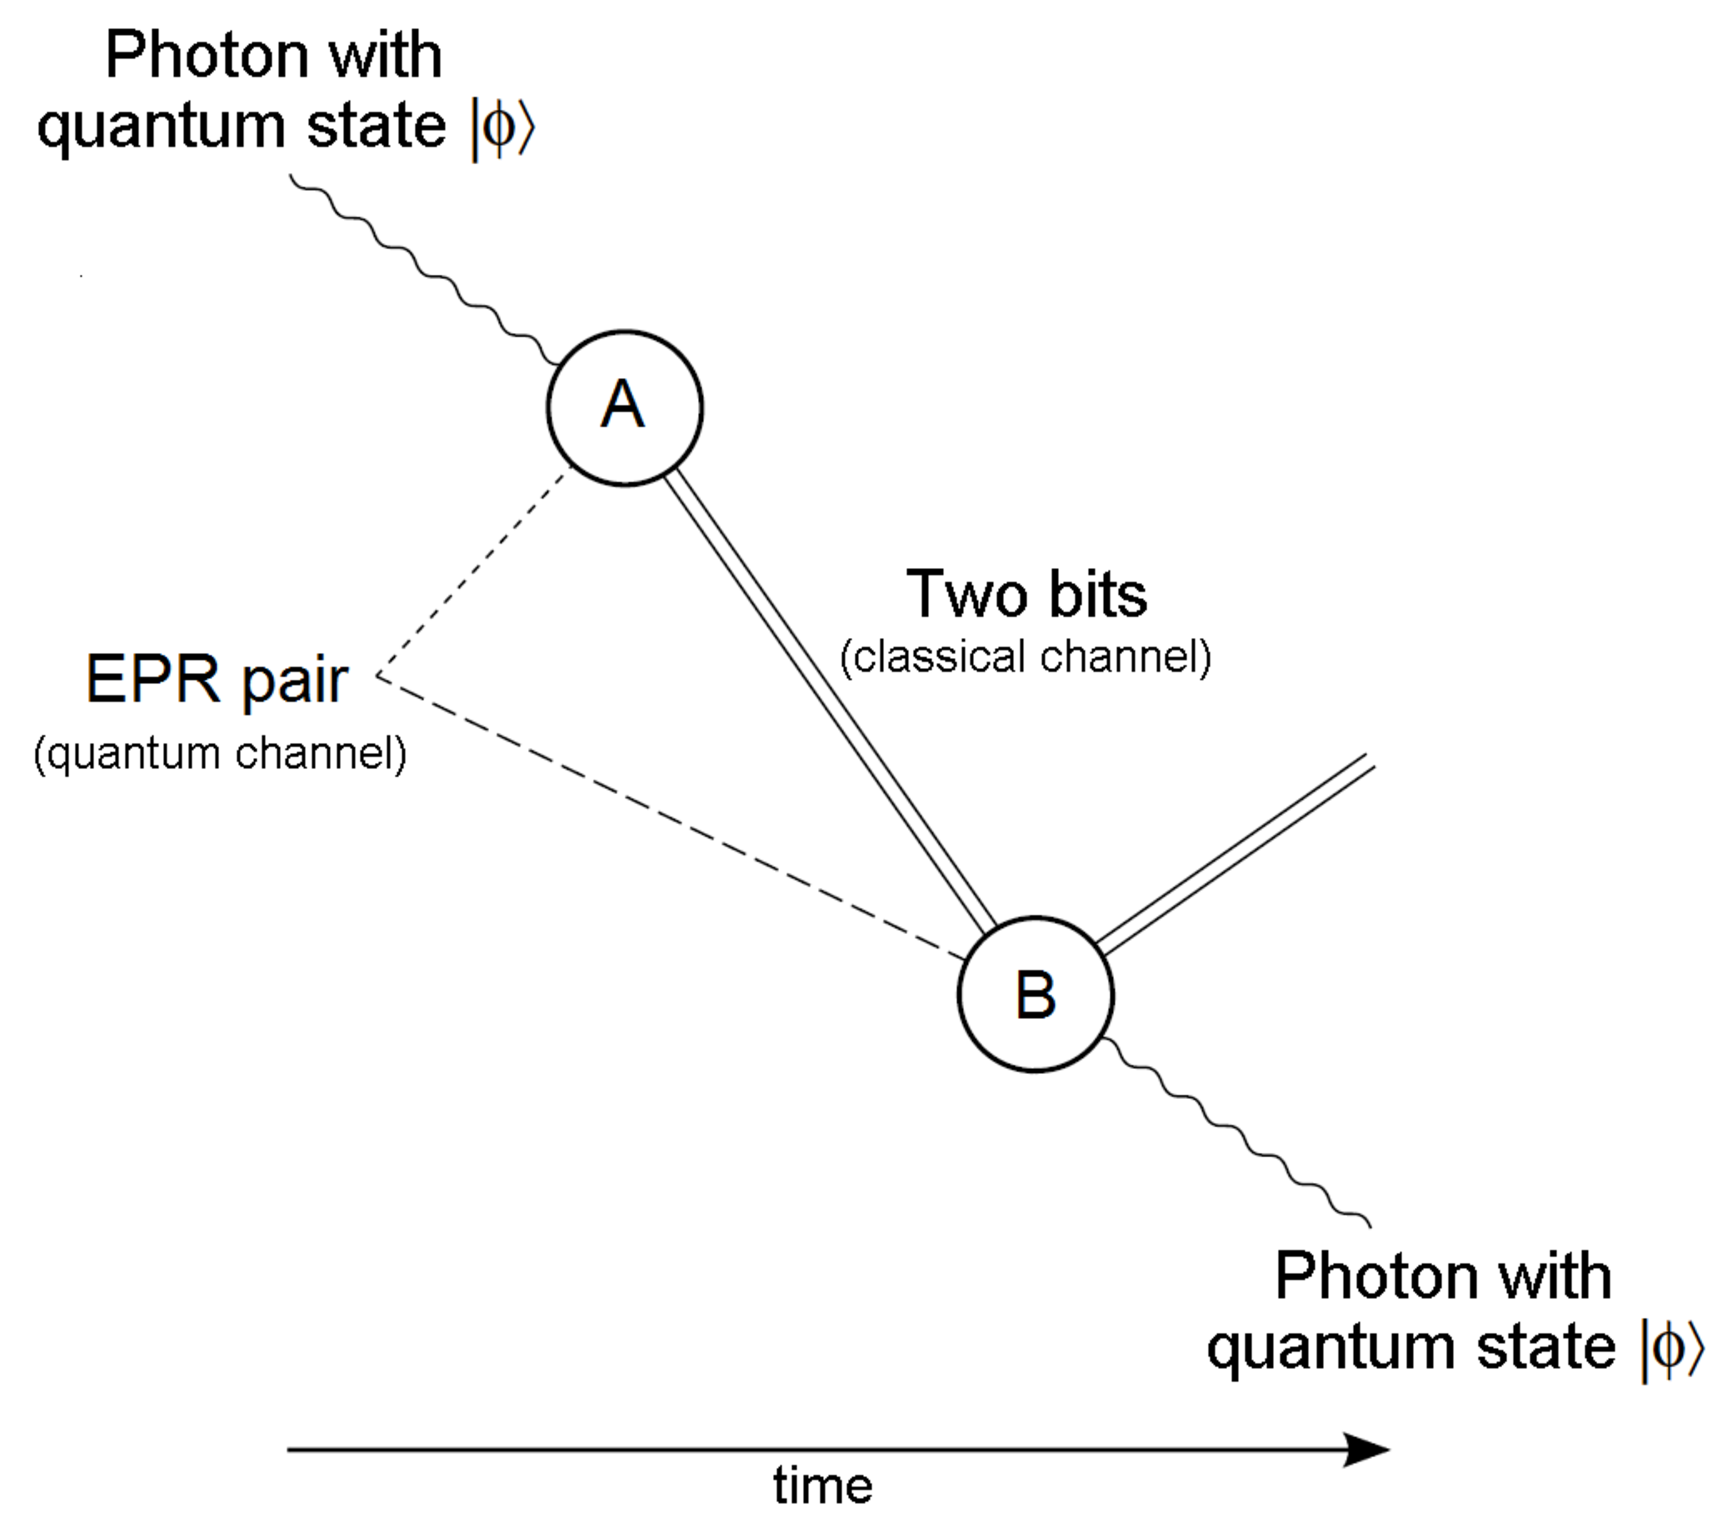
\includegraphics{epsTeleportation.eps}}
\caption{Schematic diagram for quantum teleportation.} \label{Fig:Teleport}
\end{figure}

Quantum teleportation can be regarded as a secure way to transfer information \cite{Lo1999Science}.


\section{Quantum Super dense coding}

%% week2-2
The unitary operation $\vert \psi\rangle_{AB}\to \vert \phi\rangle_{AB}$ does not necessarily indicate that $\rho_A\to E(\rho_A) = \rho_A'$ is also unitary.
The super operation $\mathcal{E}(\rho) = \sum_a M_a\rho M_a^\dagger,$ in which $\sum_a M_a M_a^\dagger=I$. (read Preskill lecture notes for more details, related to quantum channel which we will discuss in later lectures). 


%% week3-2

\section{XOR Games}

Separate boxes (e.g., 16 l.y. away), local referees each give Alice or Bob random variables. $x\in\{0,1\}\to [A] \to a\in\{0,1\}$; $y\in\{0,1\}\to [B]\to b\in\{0,1\}$. In order to win, Alice and Bob need to make sure $a\oplus b = x\cdot y$. No communication in the games, but before the game they can discuss the strategy.

Analysis: $\Pr[x\cdot y = 0] = \frac{3}{4}, \Pr[x\cdot y = 1] = \frac{1}{4}$.

 Random strategy can win with probability $\frac{1}{2}$. Always outputs same result, $a\oplus b = 0$, win with probability $\frac{3}{4}$.
 
Proof: No strategy achieves larger probability than $\frac34$. Maximize $S = \sum_{a,b,x,y} (-1)^{a\oplus b+ x\cdot y}\Pr[a,b\vert x,y]$. Note that $a$ can not depend on $y$ and $b$ can not depend on $x$, so $\Pr[a,b\vert x,y] = \Pr[a\vert x]\Pr[b\vert y]$.
\begin{eqnarray*}
S&=& \sum_{a,b,x,y}(-1)^{a+b+x\cdot y}\Pr[a\vert x]\Pr[b\vert y]\\
&=& \sum_{x,y} \sum_{a,x}(-1)^a\Pr[a\vert x]\sum_{b,y}(-1)^b \Pr[b\vert y](-1)^{xy}\\
&=& \sum_{a,x}(-1)^a \Pr[a\vert x]\sum_{b}(-1)^b\left[ \Pr[b\vert 0]+\Pr[b\vert 1](-1)^x \right]
\end{eqnarray*}

Case by case, denote the conditional expectations $A(x) = \Pr[a =0\vert x] -\Pr[a=1\vert x], B(y) = \Pr[b=0\vert y]-\Pr[b=1\vert y], A,B\in[-1,+1]$. Then $\Tr(\rho \sigma_z)\sim A$
\begin{enumerate}
\item $x\cdot y=0$: $\sum_{a,b} (-1)^{a+b}\Pr[a\vert x]\Pr[b\vert y] = \sum_{a}(-1)^a \Pr[a\vert x] \sum_b (-1)^b \Pr[b\vert y]$.
\item $x = y = 1$: $-\sum_{a}(-1)^a \Pr[a\vert 1] \sum_b (-1)^b \Pr[b\vert 1]$.
\end{enumerate} 
$S = A(0)B(0)+A(1)B(0)+A(0)B(1)-A(1)B(1) = A(0)[B(0)+B(1)]+A(1)[B(0)-B(1)] \leq 2$. Use probabilistic explanation, treat $A,B$ as random variables in $\{-1,1\}$. At least two terms are 0's. Or solve by linear optimization for continuous $A,B$ in $[-1,1]$.


Relate classical prob to quantum measurement. $x=0: A_0, \rho_A$. $\Tr(A_0 \rho_A) = A(0)$. Similar for $x=1, A_1; y=0, B_0; y=1, B_1$.

$\psi_{AB} = \ket{00}+\ket{11}$
$A_0 = \sigma_z, A_1 = \sigma_x, B_0 = \frac1{\sqrt2} (\sigma_x+\sigma_z), B_1 = \frac1{\sqrt2} (\sigma_x-\sigma_z)$.

The expectation $S = \langle A_0B_0 +A_0B_1+A_1B_0-A_1B_1\rangle$.
$\langle A_0 B_0\rangle = \Tr(\rho_{AB}\sigma_x\otimes \frac{\sigma_x+\sigma_z}{\sqrt{2}}) = \frac{1}{\sqrt2}\langle \sigma_x\otimes\sigma_x\rangle+\frac{1}{\sqrt2}\langle \sigma_x\otimes\sigma_z \rangle = \frac{1}{\sqrt2}+0$.

So $S = \frac{\sqrt2}{2}\times 3-(-\frac{\sqrt2}{2}) = 2\sqrt{2}>2$. (Why contradicts the classical results?)

%% END week3



%%%%%%%%%%%%%%%%%%%%%%%%%%%%%%%%%%%%%%%%
% choose a style
%\bibliographystyle{ieeetr}
%\bibliographystyle{unsrt}
\bibliographystyle{apsrev4-1}
%%%%%%%%%%%%%%%%%%%%%%%%%%%%%%%%%%%%%%%%


%%%%%%%%%%%%%%%%%%%%%%%%%%%%%%%%%%%%%%%%
% choose a .bib file
\bibliography{bibAdvQI}
%%%%%%%%%%%%%%%%%%%%%%%%%%%%%%%%%%%%%%%%
\end{document}
